\subsection{Testing for Weak password policy - OTG-AUTHN-007} \label{OTG-AUTHN-007}
\subsubsection{BANK-APP}
\begin{longtable}[l]{ p{2.3cm} | p{.79\linewidth} }\hline
    & \textbf{BANK-APP}
    \hfill CVSS Score: 8.5 \progressbar[filledcolor=red]{0.85}
    \\ \hline
    \textbf{Observation} & It has been observed that there is no restriction on the choice of passwords during registration. This reveals that passwords of users can be cracked and this vulnerability has been observed in the Login page. \\
    \textbf{Discovery} &
         This vulnerability was tested using the Firefox addon Fireforce. However, it did not yield right results even after multiple tries. We tested with the Brute force attack as well as the Dictionary option. Even using the Dictionary attack with a file containing just 5 passwords did not provide the right password. Tests were terminated by always giving the first word as the password. See Figure \ref{fig:password_cracking}.
         Hence we tried the THC Hydra login hacking tool and this vulnerability has been exposed. Steps are as follows.
         \begin{itemize}
             \item Open the THC Hydra terminal and enter the command in the following format. hydra -L <username list> -p <password list> <IP Address> <form parameters> <failed login message>. In our case, the command looks like: hydra -L testuser@test.com -p Top500.txt <IP-address> http-post-form  \enquote{secure-coding/public/login.php \allowbreak :email=testuser@test.com\&password=\^PASS\^  \&submit=:Invalid login credentials}.

             \item After running the exploit with the list of Top 500 passwords, the password was found in 14 secs. See Figure \ref{fig:password_cracking}.
         \end{itemize}
    \\
    \textbf{Likelihood} & Likelihood is high. The attacker can use Brute Force to crack the passwords. As there is no restriction enforced on passwords, it is quite vulnerable. In addition, with the knowledge of THC Hydra or other password cracking tools, an attacker can easily get access to user credentials. \\
    \textbf{Impact} & After gaining access to the credentials, the attacker can gain access to the victim's account and perform all operations. In case the victim happens to be an employee or administrator, the attacker can reject other users, thus causing a Denial of Service to them. The attacker can also reject all pending transactions. \\
    \textbf{Recommen\-dations} & There should be restrictions enforced on the strength of passwords such as consisting of a combination of lower \& upper-case letters, numeric and special characters and maintain a minimum length. \\ \hline
    \textbf{CVSS} &
        \begin{tabular}[t]{@{}l | l}
            Attack Vector           & \textcolor{red}{Network}\\
            Attack Complexity       & \textcolor{Green}{High} \\
            Privileges Required     & \textcolor{BurntOrange}{Low}\\
            User Interaction        & \textcolor{red}{None} \\
            Scope                   & \textcolor{red}{Changed} \\
            Confidentiality Impact  & \textcolor{red}{High} \\
            Integrity Impact        & \textcolor{red}{High}\\
            Availability Impact     & \textcolor{red}{High}
        \end{tabular}
    \\ \hline
\end{longtable}

\subsubsection{SecureBank}
\begin{longtable}[l]{ p{2.3cm} | p{.79\linewidth} }\hline
    & \textbf{SecureBank}
    \hfill CVSS Score: 8.5 \progressbar[filledcolor=red]{0.85}
    \\ \hline
    \textbf{Observation} & It has been observed that there is no restriction on the choice of passwords during registration. This reveals that passwords of users can be cracked and this vulnerability has been observed in the Login page. \\
    \textbf{Discovery} & Same as described for BANK-APP. \\
    \textbf{Likelihood} & Same as described for BANK-APP. \\
    \textbf{Impact} & Same as described for BANK-APP. \\
    \textbf{Recommen\-dations} & Same as described for BANK-APP. \\ \hline
    \textbf{CVSS} & Same as described for BANK-APP.
    \\ \hline
\end{longtable}

\begin{figure}[ht]
	\centering
	\begin{subfigure}{.45\textwidth}
		\centering
		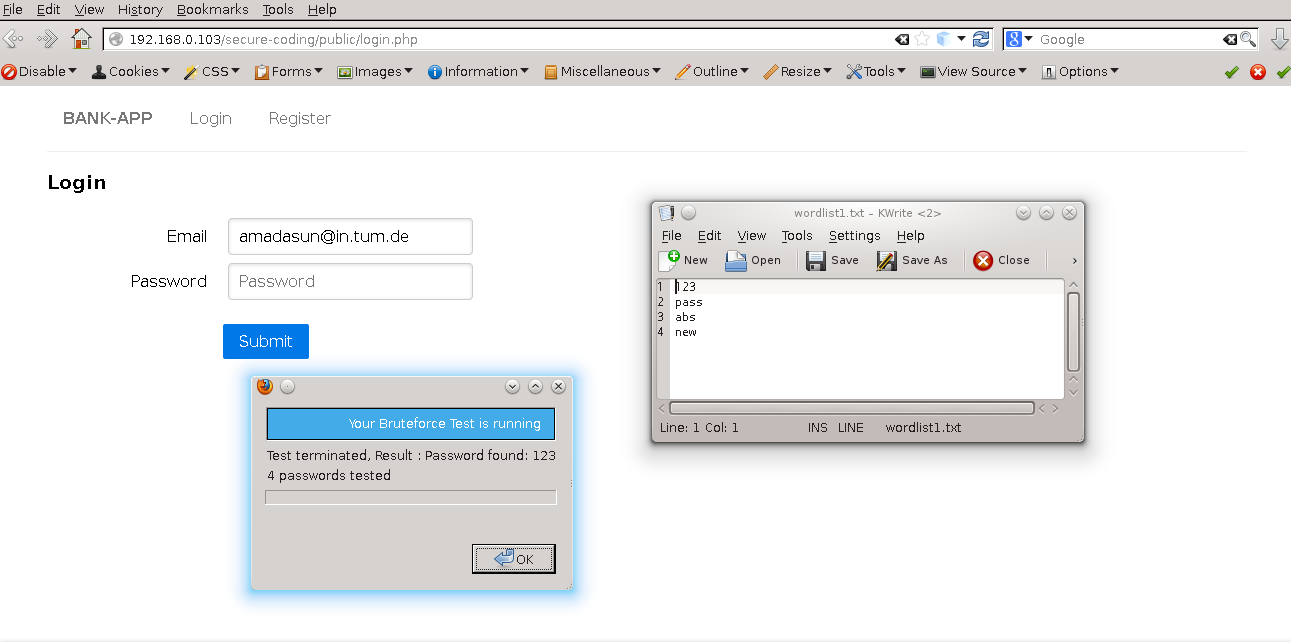
\includegraphics[width=.9\linewidth]{figures/OTG-AUTHN-007_1.png}
		\caption{Fireforce - Password cracking}
	\end{subfigure}\hfill%
	\begin{subfigure}{.45\textwidth}
		\centering
		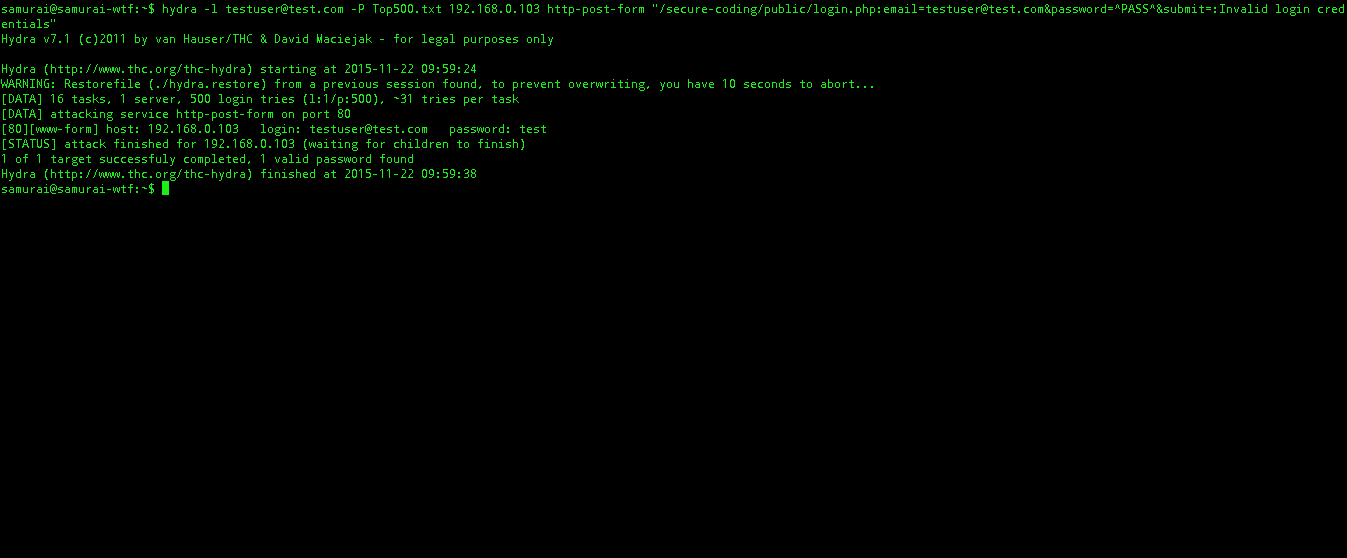
\includegraphics[width=.8\linewidth]{figures/OTG-AUTHN-007_2.png}
		\caption{THC Hydra - Password cracking}
	\end{subfigure}
	\caption{Tests for cracking password}
	\label{fig:password_cracking}
\end{figure}

\subsubsection{Comparison}
Both of the applications are vulnerable to password attacks since there is no policy behind setting passwords and no enforcement of strong passwords.
\clearpage